%! TEX program = lualatex
\documentclass[12pt]{article}
% Packages
%\usepackage[margin=1.5in]{geometry}
\usepackage{index}
\usepackage{amsbsy} % Bold math symbols
\makeindex
%\usepackage[utf8]{inputenc}
\usepackage[T1]{fontenc}
\usepackage{tcolorbox}
\tcbuselibrary{theorems}
\tcbuselibrary{skins}
\tcbuselibrary{breakable}
\usepackage{varwidth}
\usepackage{textcomp}
\usepackage{amsmath, amssymb}
\usepackage{esint}
\usepackage{titlesec}
\usepackage{xcolor}
\usepackage{titling}
\usepackage[linktocpage]{hyperref}
\usepackage{pgfplots}
\usepackage{multicol}
\setlength{\columnsep}{2em}
\usepackage{caption}
\usepackage{amsthm}
\usepackage{import}
\usepackage{cancel}
\usepackage{caption}
\usepackage{nicematrix}
\usepackage{mathrsfs}
\usepackage{mathtools}
%\usepackage{parskip}
\usepackage{enumerate}
\usepackage{graphicx}
\usepackage[italian]{babel}
\usepackage{setspace}
\setstretch{1.2}
% To reset footnote numbering each page
\usepackage[perpage]{footmisc}
\usepackage{faktor}
\usepackage{tikz-cd}
\definecolor{mastercolor}{HTML}{0c800f}
\definecolor{nred}{HTML}{bf0040}

% Titles 
\title{Appunti di\\ \vspace{.3cm} Geometria e topologia differenziale}
\author{Manuel Deodato}
\date{}




\newtheoremstyle{style}% name of the style to be used
{5pt}% measure of space to leave above the theorem. E.g.: 3pt
{5pt}% measure of space to leave below the theorem. E.g.: 3pt
{\normalfont}% name of font to use in the body of the theorem
%{15pt}% measure of space to indent
{0pt}% measure of space to indent
{\noindent\sffamily\scshape\bfseries}% name of head font
{}% punctuation between head and body
{ }% space after theorem head; " " = normal interword space
{\thmname{#1}\thmnumber{ #2}{\thmnote{ (#3)}.\ }}


\theoremstyle{style}
\newtheorem{esempio}{Esempio}[section]
\newtheorem{definizione}{Definizione}[section]
\newtheorem{prop}{Proposizione}[section]
\newtheorem{teorema}{Teorema}[section]
\newtheorem{lemma}{Lemma}[teorema]
\newtheorem{corollario}{Corollario}[teorema]
\newtheorem{osservazione}{Osservazione}[section]
\newtheorem{notazione}{Notazione}[section]
\newtheorem{esercizio}{Esercizio}[section]





\tcolorboxenvironment{definizione}{blanker,breakable,left=5mm,before skip=10pt,after skip=10pt, borderline west={.5mm}{0pt}{mastercolor}, before upper={\setlength{\parindent}{15pt}}}
\tcolorboxenvironment{lemma}{blanker,breakable,left=5mm,before skip=10pt,after skip=10pt, borderline west={.5mm}{0pt}{mastercolor}, before upper={\setlength{\parindent}{15pt}}}
\tcolorboxenvironment{teorema}{enhanced,blanker,breakable,left=5mm,before skip=10pt,after skip=10pt, borderline west={.5mm}{0pt}{mastercolor}, before upper={\setlength{\parindent}{15pt}}}
\tcolorboxenvironment{corollario}{blanker,breakable,left=5mm,before skip=10pt,after skip=10pt, borderline west={.5mm}{0pt}{mastercolor}, before upper={\setlength{\parindent}{15pt}}}
\tcolorboxenvironment{prop}{blanker,breakable,left=5mm,before skip=10pt,after skip=10pt, borderline west={.5mm}{0pt}{mastercolor}, before upper={\setlength{\parindent}{15pt}}}
\tcolorboxenvironment{esempio}{blanker,breakable,left=5mm,before skip=10pt,after skip=10pt, borderline west={.5mm}{0pt}{mastercolor}, before upper={\setlength{\parindent}{15pt}}}
\tcolorboxenvironment{esercizio}{blanker,breakable,left=5mm,before skip=10pt,after skip=10pt, borderline west={.5mm}{0pt}{mastercolor}, before upper={\setlength{\parindent}{15pt}}}
\tcolorboxenvironment{osservazione}{blanker,breakable,left=5mm,before skip=10pt,after skip=10pt, borderline west={.5mm}{0pt}{mastercolor}, before upper={\setlength{\parindent}{15pt}}}


\newenvironment{svolgimento}{\renewcommand\qedsymbol{$\blacksquare$}\begin{proof}[Svolgimento]}{\end{proof}}




%% Generic box
\newtcolorbox{eqbox}[1][]
{
colback=gray!10,
arc=0pt,
boxrule=0pt,
title=#1
}

 \newenvironment{boxenv}[1][]{
    \begin{eqbox}[#1]
    }{
   \end{eqbox}
}



%Captions
\captionsetup[figure]{font=footnotesize,labelfont=footnotesize}
\captionsetup[table]{font=footnotesize,labelfont=footnotesize}
%Titlesec
\titleformat{\section}
{\fontsize{20}{20}\scshape}
{\normalfont\color{gray}{\fontsize{80}{20}\selectfont\thesection\hspace{.2cm}\color{gray}{\vrule width 1pt}}}
{0.7em}
{}
\titlespacing*{\section}{0pt}{*2}{1cm}
\titlespacing*{\subsection}{0pt}{*5}{.5cm}
\titlespacing*{\subsubsection}{0pt}{*5}{.5cm}

\hypersetup{colorlinks,breaklinks, linkcolor=[RGB]{12,128,15}}

% Personalizza la formattazione della subsection
\titleformat{\subsection}[block]{\centering\fontsize{15}{20}\bfseries}{\color{nred}\normalfont\S\thesubsection}{.5em}{}


% Personalizza la formattazione della subsubsection
\titleformat{\subsubsection}[block]{\centering\fontsize{14}{20}\bfseries}{\color{nred}\normalfont\S\thesubsubsection}{.5em}{}

% Maketitle customization
\renewcommand{\maketitle}{
\begin{center}
{\sffamily
{\fontsize{20}{20}\selectfont\MakeUppercase\thetitle}}

\vspace{0.2in}

{\large\scshape\theauthor}
\end{center}
}

%Evaluate symbol
\DeclareMathOperator{\di}{d\!}
\newcommand*\Eval[3]{\left.#1\right\rvert_{#2}^{#3}}

%%%%%%% Numero delle equazioni in formato a.b
\numberwithin{equation}{subsection}
%%%%%

%%%%%%%%%% Personalizzazione numeri lista
\renewcommand{\theenumi}{(\arabic{enumi})}

%%%% Table of contents

\usepackage[titles]{tocloft}

\renewcommand{\cftdot}{}
\usepackage{titletoc}
%\setcounter{tocdepth}{2}

%%%%%%%%%%%%%%%% Toc style

% Personalizzazione scritta indice


% Font
\renewcommand{\textbf}[1]{\textsf{\bfseries #1}}
\usepackage[osf]{newpxtext}
\usepackage[euler-digits,euler-hat-accent]{eulervm}
\usepackage{fontspec}
\DeclareSymbolFont{operators}{OT1}{EBGaramond-TLF}{m}{n}


\newcommand{\longhookrightarrow}{\lhook\joinrel\longrightarrow}
\begin{document}
\maketitle
\vspace{7cm}
\begin{figure}[h!]
	\centering
	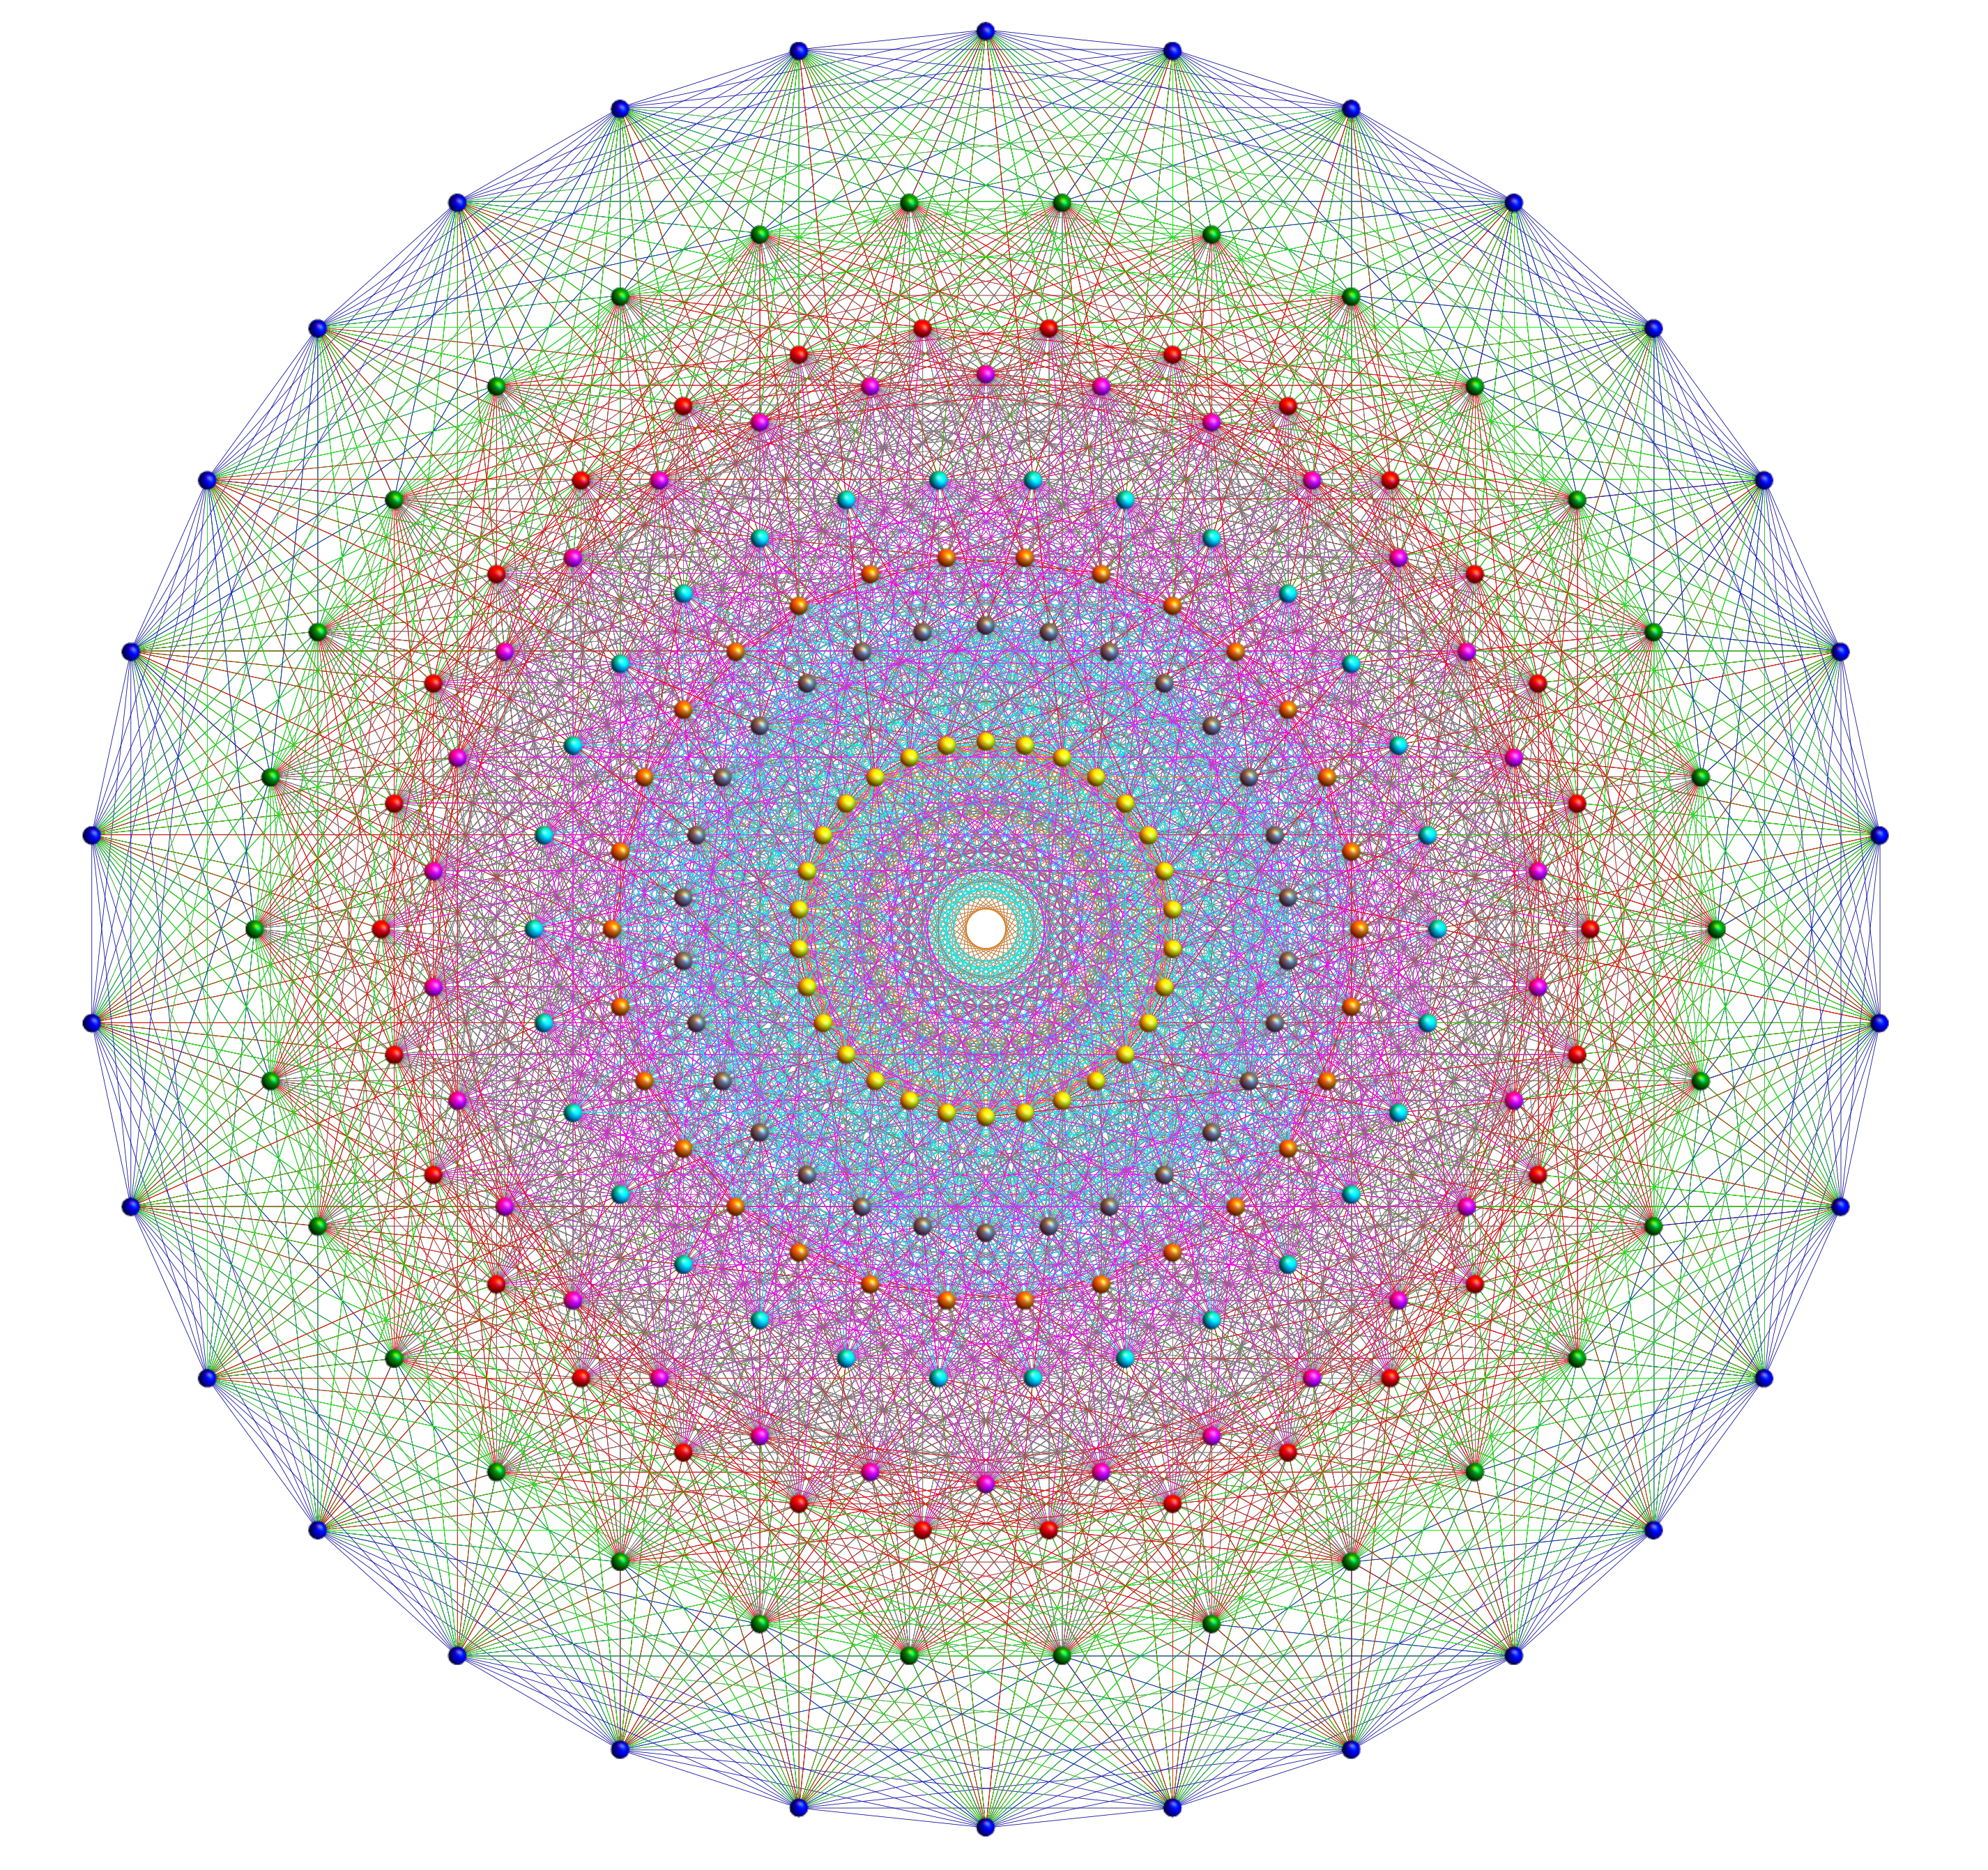
\includegraphics[width=.6\columnwidth]{front.jpg}
\end{figure}

\newpage
\tableofcontents 
\newpage
\section{Teoria delle curve}
\subsection{Introduzione}
\begin{definizione}
	[Curva parametrizzata]
	Una \textit{curva paramtrizzata} \`e un'applicazione $\alpha  : I\subset \mathbb{R} \to \mathbb{R}^3$ di classe $C^\infty(I)$, con $I$ intervallo aperto.
	Data $t\in I$, si pu\`o scrivere in componenti come
	\[
	\alpha (t) = (x(t),y(t),z(t))
	\] 
	con $x,y,z:I\to \mathbb{R}$ tutte di classe $C^\infty(I)$.
\end{definizione}
\begin{osservazione}
La necessit\`a di definire la curva su un aperto, o quantomeno di poter estendere l'intervallo di definizione ad un aperto, deriva dal fatto che, in questo modo, si pu\`o effettivamente parlare di derivata piena anche per gli estremi, potendo trovare, infatti, un aperto che contiene interamente i punti di frontiera dell'intervallo di definizione.
Se non si avesse questa possibilit\`a, nel caso di $\alpha :[a,b] \subset \mathbb{R}\to \mathbb{R}^3$, per esempio, non si potrebbe calcolare la derivata tradizionale in $a$, o $b$, perch\'e si potrebbe solamente calcolare il limite destro o sinistro.
\end{osservazione}
\noindent Si nota che, nel caso in cui $I$ non fosse aperto, si estende l'intervallo di definizione ad $A \supset I$ aperto.

Si parla di \textit{traccia} della curva in riferimento all'immagine che genera dell'intero intervallo: $\operatorname{Tr} \alpha  = \alpha (I)$.
La traccia rappresenta l'unione di ciascun punto di $\alpha (t) \in \mathbb{R}^3, \ \forall t \in I$.
Per \textit{velocit\`a} della curva, invece, si intende la grandezza\footnote{Questa \`e ben definita perch\'e si sta operando in uno spazio vettoriale, con $\alpha (t+h) - \alpha (t)$ giustificata dall'operazione di somma dello spazio e divisione per $h$ data dalla moltiplicazione per uno scalare.}
\begin{equation}
	\alpha '(t) = \lim_{h \to 0} \frac{\alpha (t + h) - \alpha (t)}{h} = \big(x'(t),y'(t),z'(t)\big)
\end{equation}
In realt\`a, questo rappresenta il \textit{vettore velocit\`a}, mentre la velocit\`a vera e propria \`e data dalla sua norma $\left\lVert \alpha' (t) \right\rVert $.
\begin{esempio}
	[Retta parametrizzata]
	Siano $P,Q \in \mathbb{R}^3$, con $P\neq Q$, due punti dello spazio; si definisce, allora, \textit{retta parametrizzata} la curva 
	\[
		\alpha :
		\begin{array}
			{c c c}
			[0,1] &\longrightarrow & \mathbb{R}\\
			t &\longmapsto & P + t(Q-P) = P+t \overrightarrow{PQ}
		\end{array}
	\] 
La sua traccia \`e la retta affine passante per $P$ e $Q$, e ha vettore velocit\`a $\alpha '(t) = \overrightarrow{PQ}$, da cui $\left\lVert \alpha '(t) \right\rVert = \lVert \overrightarrow{PQ} \rVert$, che \`e costante.
\end{esempio}
\begin{esempio}
	[Circonferenza parametrizzata]
Dato $a\in \mathbb{R}$, con $a > 0$, si definisce \textit{circonferenza parametrizzata} come 
\[
\alpha:
	\begin{array}
		{c c c}
		[0,2\pi] &\longrightarrow & \mathbb{R}^3\\
		t &\longmapsto & (a \cos t, a \sin t , 0)
	\end{array}
\] 
il cui vettore velocit\`a \`e dato da $\alpha '(t) = (-a\sin t, a \cos t, 0)$, che non risulta costante, mentre la sua velocit\`a $\left\lVert \alpha ' \right\rVert = a >0$ s\`i.
La traccia corrisponde ad una circonferenza nel piano $z=0$, di centro l'origine e raggio $a$.
\end{esempio}
\subsection{Riparametrizzazione di una curva}
Sia $\alpha : [a,b]\to\mathbb{R}^3$ una curva parametrizzata; una sua \textit{riparametrizzazione} \`e data dalla coppia di mappe $h:[a,b]\to [c,d] \subseteq \mathbb{R}$ e $\beta : [c,d]\to \mathbb{R}^3$ tali che il diagramma
\[
\begin{tikzcd}
	\left[ a,b \right]  & & \mathbb{R}^3\\
	\\
	\left[ c,d \right] 
	\arrow[from=1-1, to=1-3, "\displaystyle \alpha "]
	\arrow[from=1-1,to=3-1,"\displaystyle h"']
	\arrow[from=3-1,to=1-3,"\displaystyle \beta"']
\end{tikzcd}
\] 
commuta, quindi si ha $\beta (h(t)) = \alpha (t)$. 
Perch\'e questo sia verificato, si assume che $h \in C^\infty([a,b])$ e $h'(t) \neq 0, \ \forall t \in [a,b]$; in questo modo, $\exists h^{-1}$ di classe $C^\infty$ tale che $\beta = \alpha \circ h^{-1}$, quindi anche $\beta $ risulta liscia ed \`e verificata la relazione $(\beta \circ h)(t) = \alpha (t)$, con $\operatorname{Tr} \alpha =\operatorname{Tr} \beta $.

Ora si definisce la lunghezza di una curva; se ne giustifica la definizione tramite il seguente ragionamento.
Sia dato $[a,b] \subset \mathbb{R}$ un intervallo e sia $P \in \mathcal{P} ([a,b])$ una sua partizione, tale che $a = t_0 < t_1 < \ldots<t_{k-1} <t_k = b$; allora la lunghezza di una curva $\alpha  : [a,b] \to \mathbb{R}^3$ approssimata a tale partizione \`e data da:
\begin{equation}
	L(\alpha , P) = \sum_{i=0}^{k-1} \left\lVert \alpha (t_{i+1}) - \alpha (t_i) \right\rVert 
\end{equation}
Si nota, dunque, che la lunghezza effettiva della curva coincide con
\begin{equation}
	\sup_{P \in \mathcal{P}([a,b]) } L(\alpha ,P) = \int_{a} ^b \left\lVert \alpha' (u) \right\rVert du
\end{equation}
\begin{definizione}
	[Lunghezza d'arco]
	Sia $\alpha  : [a,b] \subset \mathbb{R}\to \mathbb{R}^3$ una curva; si definisce \textit{lunghezza d'arco} la funzione
	\[
	s :
	\begin{array}
		{c c c}
		[a,b] & \longrightarrow &\mathbb{R}\\
		t & \longmapsto &\displaystyle  \int_{a} ^t \left\lVert \alpha '(u) \right\rVert du
	\end{array}
	\] 
	La lunghezza dell'intera curva $\alpha $ \`e data da $L(\alpha ) = s(b)$.
\end{definizione}
\begin{osservazione}
Si nota che per $\alpha : [0,+\infty) \to \mathbb{R}^3$, con $\alpha  (t) = \big(a \cos t, a \sin t, 0\big)$, valendo $\left\lVert \alpha '(t) \right\rVert = a$, si ha:
\[
s(t) = a \int_{0} ^t du = ta \implies s (2\pi) = 2\pi a
\] 
\end{osservazione}
\noindent Vale la pena chiedersi se $L(\alpha )$ sia indipendente dalla sua parametrizzazione, cio\`e se $L(\alpha ) = L(\beta )$, se $\beta $ \`e una riparametrizzazione di $\alpha $; questo si vede facilmente per conto diretto.
\begin{proof}
	Se $\alpha (t) = \beta (h(t))$, allora $\alpha '(t) = \beta '(h(t)) h'(t)$, quindi
	\[
	L(\alpha ) = \int_{a} ^b \left\lVert \alpha '(t) \right\rVert dt = \int_{a} ^b \lvert h'(t) \rvert \left\lVert \beta '(h(t)) \right\rVert dt
	\] 
	Ora si distinguono due casi: essendo $h'(t)\neq 0, \ \forall t$, si pu\`o avere o $h'(t) <0$, o $h'(t) > 0$. 
	Nel primo caso, si ha $h'(t) < 0$, quindi $\lvert h'(t) \rvert = - h'(t)$, con $h(a) = d$ e $h(b) = c$; nel secondo caso, $\lvert h'(t) \rvert =h'(t)$, con $h(a) = c$ e $h(b) = d$.
	Si trova, per $s = h(t)$, rispettivamente:
	\[
	\begin{cases}
		\displaystyle -\int_{d} ^c h'(t) \left\lVert \beta '(h(t))  \right\rVert dt = \int_{c} ^d \left\lVert \beta '(s) \right\rVert ds = L(\beta )\\
		\\
		\displaystyle \int_{c} ^d h'(t) \left\lVert \beta '(h(t)) \right\rVert dt = \int_{c} ^d \left\lVert \beta '(s) \right\rVert ds = L(\beta )
	\end{cases}
	\] 
In entrambi i casi, dunque, si ottiene $L(\alpha ) = L(\beta )$.	
\end{proof}
\noindent Ora si introduce una particolare riparametrizzazione, talvolta nota col nome di \textit{riparametrizzazione canonica}, o \textit{naturale}; per poterla definire, \`e necessario che $\alpha $ soddisfi la seguente condizione.
\begin{definizione}
	[Curva regolare]
	Una curva parametrizzata $\alpha : I \subset \mathbb{R} \to \mathbb{R}^3$ \`e detta \textit{regolare} se $\alpha '(t) \neq 0, \ \forall t \in I$.
\end{definizione}
\noindent Si considera, quindi, una curva regolare $\alpha :[a,b] \to \mathbb{R}^3$; visto che $s(t) = \int_{a} ^t \left\lVert \alpha '(u) \right\rVert du$, allora $s'(t) = \left\lVert \alpha '(t) \right\rVert >0$.
Si pu\`o pensare alla lunghezza d'arco come $s : [a,b] \to [0, L(\alpha )]$, che, essendo monotona perch\'e si \`e appena osservato che $s'(t) > 0$, allora ha anche inversa $t : [0,L(\alpha )]\to [a,b]$.
\`E, quindi, possibile definire la funzione 
\begin{equation}
	\beta = \alpha \circ t : [0,L(\alpha )]\to \mathbb{R}^3
\end{equation}
tale che $\operatorname{Tr} (\beta )=\operatorname{Tr} (\alpha ) $ e $\beta (s) = \alpha (t(s))$, per cui
\[
\beta '(s) = \alpha '(t(s)) t'(s) = \frac{\alpha '(t(s))}{s'(t(s))} = \frac{\alpha '(t(s))}{\left\lVert \alpha '(t) \right\rVert }
\] 
per cui $\left\lVert \beta '(s) \right\rVert =1$.
\begin{definizione}
	[Curva p.l.a.]
	Se $\alpha :I\to\mathbb{R}^3$ \`e una curva tale che $\left\lVert \alpha '(t)\right\rVert = 1 , \ \forall t \in I$, allora si dice che \`e \textit{parametrizzata tramite lunghezza d'arco}, o pla.
\end{definizione}
\begin{osservazione}
In base a quanto detto prima, ogni curva regolare \`e \textit{riparametrizzabile tramite lunghezza d'arco}.
\end{osservazione}
\begin{osservazione}
	[Non unicit\`a della versione pla]
	Data una curva regolare $\alpha  : I \to \mathbb{R}^3$, la riparametrizzazione tramite lunghezza d'arco non \`e univoca ma dipende dall'estremo inferiore di integrazione della lunghezza d'arco $s(t)$; se, infatti, $a,b \in I$ con $a < b$:
	\[
	s_a (t) = \int_{a} ^t \left\lVert \alpha '(u) \right\rVert du \hspace{1cm}s_b (t) \int_{b} ^t \left\lVert \alpha '(u) \right\rVert du
	\] 
	Le due, per\`o, differiscono solo per una costante perch\'e
	\[
	s_a(t) = \int_{a} ^b \left\lVert \alpha '(u) \right\rVert du + \int_{b} ^t \left\lVert \alpha '(u) \right\rVert du = \text{cost.} + s_b(t)
	\] 
	Questa differenza per una costante non influir\`a sulla trattazione del riferimento di Frenet perch\'e si lavora con derivate e la costante sparisce.
\end{osservazione}
\begin{esempio}
	[Elica]
Sia $a > 0$; allora la mappa
\[
\varphi :
\begin{array}
	{c c c}
	\mathbb{R}^2 & \longrightarrow & \mathbb{R}^3\\
	(u,z) &\longmapsto & (a \cos u , a \sin u , z)
\end{array}
\] 
definisce un cilindro di raggio $a$ attorno all'asse $z$.
Preso $b > 0$ e presi i punti $\left\{ (t,bt) \right\} _{t \in \mathbb{R}} $, relativi ad una retta passante per l'origine, aperto, si pu\`o definire la curva 
\[
\alpha (t) = \varphi (t,bt) = (a \cos t , a \sin t , bt)
\] 
che descrive un'\textit{elica destrorsa}, visto che si \`e preso $b>0$\footnote{Fosse stato $b<0$, sarebbe stata un'\textit{elica sinistrorsa}.}, di raggio $a$ e passo $b$.
Si nota che
\[
\alpha '(t) = (-a \sin t, a \cos t , b) \implies \left\lVert \alpha '(t) \right\rVert =\sqrt{a^2 + b^2} > 0, \ \forall t \in \mathbb{R}
\] 
da cui $\alpha $ \`e regolare. 
Restringendola a $[0,+\infty)$, cio\`e considerando $\alpha : [0,+\infty) \to \mathbb{R}^{3} $, si ha:
\[
	s(t) = \int_{0} ^t \sqrt{a^2 + b^2 }  du = t(s) \sqrt{a^2 + b^2} \implies t(s) = \frac{s}{\sqrt{a^2 +b^2}}
\] 
quindi:
\[
\begin{split}
		 \beta (s) &= \alpha (t(s)) = \alpha  \left(\frac{s}{\sqrt{a^2 + b^2} }\right) \\
	&= \left(a \cos \left(\frac{s}{\sqrt{a^2+b^2} }\right) , a\sin \left(\frac{s}{\sqrt{a^2 + b^2} }\right),\frac{bs}{\sqrt{a^2 + b^2} } \right)
	\end{split} 
\] 
con $\beta $ pla e, conseguentemente, $\beta (\mathbb{R}) = \operatorname{Tr} (\beta ) = \operatorname{Tr} (\alpha ) = \alpha (\mathbb{R})$.
\end{esempio}
\begin{esempio}
	[Ellisse]
	Siano $a,b \in \mathbb{R}\setminus\left\{ 0 \right\} $ e sia 
	\[
	\mathcal{E} _{a,b} = \left\{ (x,y,0) \in \mathbb{R}^3  \ \bigg\lvert \ \frac{x^2}{a^2} + \frac{y^2}{b^2} = 1\right\} \subset \mathbb{R}^3
	\] 
	Si vuole definire una curva $\alpha $ tale che $\operatorname{Tr} \alpha = \mathcal{E} _{a,b} $
\end{esempio}
	\begin{svolgimento}
		Si nota che $(x /  a , y / b) \in S^1$, cio\`e
	\[
	\frac{x}{a} = \cos t \hspace{1cm}\frac{y}{b} = \sin t
	\] 
	con $S^1$ circonferenza unitaria e $t\in [0,2\pi)$.
	Sia, allora
	\[
\alpha :
	\begin{array}
		{c c c}
		[0,2\pi) &\longrightarrow & \mathbb{R}^3\\
		t & \longmapsto & (a \cos t , b \sin t, 0)
	\end{array}
	\] 
 e si vede che $\operatorname{Tr} \alpha  = \mathcal{E} _{a,b} $.

	\end{svolgimento}
\begin{esempio}
Sia 
\[
\mathcal{C}  = \left\{ (x,y,0) \in \mathbb{R}^3  \mid y^2 = x^3 \right\}  \subset \mathbb{R}^3
\] 
Si vuole costruire $\alpha $ tale che $\operatorname{Tr}\alpha  = \mathcal{C} $.
\end{esempio}
\begin{svolgimento}
	Se si considera la secante $y = tx$, allora $t^2 x^2 = x^3$, ossia $x= t^2$ e $y = t^3$.
	Ne segue che la curva che soddisfa la richiesta \`e $\alpha (t) = (t^2 , t^3,0)$.
\end{svolgimento}
\begin{esempio}
Sia 
\[
\mathcal{C}  = \left\{ (x,y,0)  \mid y^2 = x^3 + x^2 \right\} \subset \mathbb{R}^3
\] 
Si vuole costruire una curva $\alpha $ tale che $\operatorname{Tr} \alpha  = \mathcal{C} $.
\end{esempio}
\begin{svolgimento}
	Si considera, come prima, $y=tx $, da cui $x^3 + x^2(1-t^2) = 0$, e si vede che $x = t^2 - 1$ e $y=t^3 -t$, quindi $\alpha (t) = (t^2 - 1, t^3-t,0)$.
\end{svolgimento}
\noindent Per quanto in linea teorica se $\alpha $ \`e una curva regolare, allora si pu\`o riparametrizzare tramite lunghezza d'arco, questo non \`e praticamente fattibile in ogni singolo caso; se, per esempio, si considera $\alpha (t) = (t,t^2,t^3)$, si ha $\alpha '(t) = (1,2t,3t^2)$, che, dunque, \`e regolare, ma data
\[
s(t) = \int_{0} ^t \sqrt{1 + 4u^2 + 9u^4} du
\] 
non si \`e in grado di trovare un'espressione per $t(s)$ perch\'e la primitiva di $s$ non \`e scrivibile in termini di funzioni elementari.
\subsection{Riferimento ed equazioni di Frenet}
\begin{definizione}
	[Versore tangente]
	Data una curva riparametrizzabile $\alpha :I \to \mathbb{R}^3$ e la sua riparametrizzazione tramite lunghezza d'arco $\beta (s)$, si definisce il \textit{versore tangente} ad $\alpha $ come $T(s) = \beta '(s)$.
\end{definizione}
\begin{definizione}
	[Curvatura]
	Data una curva pla $\beta :I\to \mathbb{R}^3$ e il suo versore tangente $T(s)$, allora se ne definisce la \textit{curvatura} come
	\[
	k (s) = \left\lVert T'(s) \right\rVert 
	\] 
\end{definizione}
\noindent Ora si ricavano il riferimento di Frenet e le equazioni di Frenet.
Per poter definire il riferimento di Frenet e ricavare, conseguentemente, le equazioni di Frenet, \`e necessario imporre ulteriori condizioni sulle curve in esame; la condizione operativa necessaria \`e la seguente.
\begin{definizione}
	[Curva di Frenet]
	Una curva regolare $\alpha:[a,b]\to\mathbb{R}^3 $ \`e detta \textit{di Frenet} se la sua pla $\beta = \alpha  \circ t:[0,L(\alpha )]\to \mathbb{R}^3$ \`e tale che $k(s) >0, \ \forall s \in [0,L(\alpha )]$.
\end{definizione}
\begin{lemma}\label{lemdif}
	Se $f, g : I \to \mathbb{R}^{3} $ sono due mappe, allora 
	\[
	\left(f(t)\cdot g(t)\right) ' = f'(t) \cdot g(t) + f(t) \cdot g'(t)
	\] 
\end{lemma}
	\begin{proof}
		Si ha
		\[
		f(t) \cdot g(t) = \sum_{i=1}^{3} f_i(t) g_i(t)
		\] 
	quindi
	\[
	\left(f(t)\cdot g(t)\right) ' = \sum_{i=1}^{3} \left[ f_i'(t)g_i(t) + f_i(t) g_i'(t) \right] 
	\] 
	\end{proof}
\noindent Data $\alpha : I \to \mathbb{R}^3$ una curva di Frenet e $T(s) = \beta '(s)	$ il suo versore normale, con $\beta $ versione pla di $\alpha $, si nota che $T'(s)$ non \`e, in generale un versore e 
\[
1 = \left\lVert T(s) \right\rVert ^2 = T(s) \cdot T(s) \implies \left[ T(s) \cdot T(s) \right] ' = 2T'(s) \cdot T(s) = 0 \implies T'(s) \perp T(s) 
\] 
Avendo assunto $\alpha $ di Frenet, significa che $k_\alpha  (s) \neq 0$, quindi $T'(s)$ \`e normalizzabile e si ottiene un versore ortogonale a $T(s)$.
Usando questo versore e $T(s)$, tramite il prodotto vettore, se ne pu\`o definire un terzo; allora si ha la seguente definizione.
\begin{definizione}
	[Versori normale e binormale]
	Dato $T(s)$ versore tangente di una curva di Frenet $\alpha : I \to \mathbb{R}^3$, si definiscono $N(s) = T'(s) / \left\lVert T'(s) \right\rVert $ \textit{versore normale principale} e $B(s) = T(s) \times N(s)$ \textit{versore binormale}.
\end{definizione}
\noindent Evidentemente, si ha $\left\lVert N(s) \right\rVert =\left\lVert B(s) \right\rVert  = 1 $ e $T(s) \cdot N(s) = T(s) \cdot B(s) = N(s) \cdot B(s) =  0 $.
Ne segue che $\big(T(s),N(s),B(s)\big), \ \forall s \in I$ forma una base ortonormale di $\mathbb{R}^3$, nota col nome di \textbf{riferimento di Frenet}.
Per definizione di $N(s)$, si ottiene la \textbf{I equazione di Frenet}:
\begin{boxenv}[]
\begin{equation}
	T'(s) = k(s) N(s)
\end{equation}
\end{boxenv}
\noindent Si nota che, essendo un versore, si ha $N(s) \cdot N(s) = 1$, quindi $N'(s) \cdot N(s) = 0$ (per lo stesso ragionamento fatto per $T(s)$), dunque $N'(s) \in \langle T(s) , B(s) \rangle$; inoltre, essendo $T(s)\cdot N(s) = 0$, si ha 
\[
	T'(s) \cdot N(s) +T(s)\cdot  N'(s)=k(s) \underbracket{N(s) \cdot N(s)}_{=1}  +T(s)\cdot  N'(s) = 0 
\] 
perci\`o si trova $ \tau (s)$ tale per cui 
\begin{boxenv}[]
\begin{equation}
	N'(s) = -k(s)  T(s) + \tau (s)  B(s)
\end{equation}
\end{boxenv}
\noindent Questa \`e nota come \textbf{II equazione di Frenet}.
\begin{definizione}
	[Torsione]
	Data una curva regolare $\alpha :I\to\mathbb{R}^3$ e $\beta $ la sua pla, si definisce $\tau (s)$ come la \textit{torsione} di $\beta $ nel punto $s$.
\end{definizione}
\noindent Ripetendo lo stesso ragionamento, si ha $B(s) \cdot B(s) = 1 \Rightarrow B'(s) \cdot B(s) = 0$, da cui $B'(s) \in \langle T(s),N(s) \rangle$ e, essendo $N(s) \cdot B(s) = 0$, dalla derivata di $T(s) \cdot B(s) = 0$, si ha
\[
	T'(s) \cdot B(s) + T(s) \cdot B'(s) = k(s) \underbracket{N(s) \cdot B(s)}_{=0}  + T(s) \cdot B'(s) = 0
\] 
quindi $B'(s) \in \langle N(s) \rangle$.
Usando $T(s) \cdot B(s) = 0 $ e derivando $N(s) \cdot B(s) = 0$, si ottiene
\[
	\begin{split}
		N'(s) \cdot B(s) + N(s) \cdot B'(s) &= (- k(s) T(s) + \tau (s) B(s) )\cdot B(s) + N(s) \cdot B'(s) \\
		&= \tau (s) \underbracket{B(s)\cdot B(s)}_{=1}  + N(s)\cdot B'(s) = 0 
	\end{split}
\] 
cio\`e
\begin{boxenv}[]
\begin{equation}
	B'(s) = - \tau (s) N(s)
\end{equation}
\end{boxenv}
\noindent che \`e nota come \textbf{III equazione di Frenet}.
Ricapitolando, le equazioni di Frenet stabiliscono delle relazioni tra le derivate dei versori ortonormali del riferimento di Frenet e i versori stessi e sono:
\begin{boxenv}[]
\begin{equation}
	\begin{cases}
		T'(s) = k(s) N(s)\\
		N'(s) = - k(s) T(s) + \tau (s) B(s)\\
		B'(s)=-\tau (s) N(s)
	\end{cases}
\end{equation}
\end{boxenv}
\noindent Ora si applicano i concetti visti alle curve studiate nella sezione precedente.
\begin{esempio}
	Sia $\alpha (t) = P + t \overrightarrow{PQ}$ una curva parametrizzata (con $P,Q \in \mathbb{R}^3$ e $P\neq Q$). 
	Si ha $\alpha '(t) = \overrightarrow{PQ}$, quindi la curva \`e regolare, quindi se ne pu\`o trovare una pla:
	\[
		s(t) = \int_{a} ^t \lVert \overrightarrow{PQ} \rVert du= t \lVert \overrightarrow{PQ} \rVert \implies t = \frac{s}{\lVert \overrightarrow{PQ} \rVert }
	\] 
	quindi si ha $\beta (s) = P + s \frac{\overrightarrow{PQ}}{\lVert \overrightarrow{PQ} \rVert }$. 
	Allora il versore tangente \`e dato da 
	\[
	T(s) = \beta '(s) = \frac{\overrightarrow{PQ}}{\lVert \overrightarrow{PQ} \rVert } \implies T'(s) = 0 
	\] 
	perci\`o $k(s) = 0$ e, quindi, $\alpha $ non \`e una curva di Frenet perch\'e non ha curvatura positiva.
\end{esempio}
\begin{esempio}
Per $a>0$, sia $\alpha (t) = (a \cos t, a \sin t, 0)$ una circonferenza parametrizzata di raggio $a$.
Evidentemente, si pu\`o vedere come un caso particolare di elica parametrizzata per $b=0$, quindi si pu\`o fare uso del risultato trovato in precedenza:
\[
	\begin{split}
		&\beta (s) = \left(a \cos \left(\frac{s}{a}\right) , a\sin \left(\frac{s}{a}\right),0 \right)\implies T(s) = \left(- \sin \frac{s}{a}, \cos \frac{s}{a},0 \right) \\
		&\Rightarrow T'(s) = \underbracket{\frac{1}{a}}_{k(s)}  \underbracket{\left(-\cos \frac{s}{a},- \sin \frac{s}{a},0\right) }_{N(s)} 
	\end{split}
\] 
Si conclude che $N(s)\perp z$ e punta proprio verso $z$; inoltre, la circonferenza parametrizzata \`e una curva di Frenet perch\'e ha curvatura positiva, essendo $1 / a > 0 $ perch\'e $a > 0 $ per assunzione.
Infine:
\[
	\begin{split}
		&B(s) = \begin{pmatrix} -\sin s / a \\ \cos s / a \\ 0  \end{pmatrix} \times \begin{pmatrix} - \cos s / a\\ - \sin s / a \\ 0  \end{pmatrix} = \begin{pmatrix} 0 \\0 \\ 1 \end{pmatrix} \\
		&\Rightarrow -\tau (s) N(s) = B'(s) = 0 \implies \tau (s) = 0 
	\end{split}
\] 
\end{esempio}
\begin{esempio}
Si considera l'elica parametrizzata $\alpha = (a\cos t , a \sin t, bt)$, con raggio $a\in \mathbb{R}^{>0} $ e passo $b \in \mathbb{R}$.
La sua pla \`e gi\`a stata ricava; dato $c = \sqrt{a^2 + b^2} $, si ottiene:
\[
	\beta (s)= \left(a \cos \left(\frac{s}{\sqrt{c} }\right) , a\sin \left(\frac{s}{\sqrt{c} }\right),\frac{b}{\sqrt{c} } s\right)
\] 
da cui
\[
	T(s) = \frac{1}{c}\left(-a \sin \frac{s}{c}, a \cos \frac{s}{c}, b\right) \implies T'(s) = \underbracket{\frac{a}{c^2}}_{k(s)} \underbracket{\left(-\cos \frac{s}{c},- \sin \frac{s}{c},0\right) }_{N(s)} 
\] 
quindi, come nel caso della circonferenza, $N(s)\perp z$ e punta verso di esso.
Si ha:
\[
B(s) = \frac{1}{c} \begin{pmatrix} - a \sin s / c\\ a \cos s / c\\ b  \end{pmatrix} \times \begin{pmatrix} - \cos s / c \\ - \sin s / c \\ 0  \end{pmatrix} = \frac{1}{c} \begin{pmatrix} b \sin s / c \\ - b \cos  s / c \\ a  \end{pmatrix} 
\] 
Inoltre:
\[
	N'(s) = - k(s) T(s) +\tau (s) B(s) \implies \tau (s) = N'(s) \cdot B(s) =  \frac{b}{c^2}
\] 
Da questo, si vede che
\begin{itemize}
	\item se $b>0$, allora l'elica \`e destrorsa e $\tau (s) >0$,
	\item se $b<0$, allora l'elica \`e sinistrorsa e $\tau (s) < 0 $,
	\item se $b=0$, si ha una circonferenza e $\tau (s) = 0 $, con $k(s) = 1 / a$.
\end{itemize}
Fissando $a$, si nota che, per $b \to \pm \infty$, si ha $\tau (s) \to 0$ e $k(s) = a / (a^2 + b^2) \to 0 $.
\end{esempio}
\begin{prop}
	Sia $\alpha  : I \to \mathbb{R}^3$ una curva regolare; allora $k_\alpha = 0 \iff \alpha (I)$ \`e contenuta in una retta.
\end{prop}
	\begin{proof}
		Si divide la dimostrazione nelle due implicazioni.
		\begin{itemize}
			\item ($\Leftarrow$) Se $\alpha (I) \subseteq P+ \langle v \rangle$, per $v$ versore generico, si considera la sua versione pla $\alpha (I) = \beta (J) \subseteq P+\langle v \rangle$; allora $\beta = P + f(s) v$ e $\beta '=f'(s) v$, con $f'(s)=\pm 1$ perch\'e $\left\lVert \beta ' \right\rVert = 1$. 
				Ne segue che:
				\[
				T(s) = \beta '(s) = f'(s) v = \pm v \implies T'(s) = 0 \implies k_\alpha(s) = 0 
				\] 
			\item ($\Rightarrow $) Sia $\left\lVert T'(s) \right\rVert = k_\alpha (s) = 0 $, quindi $T(s) = \beta '(s) = v $, per qualche $v \in \mathbb{R}^3$.
				Allora si deve avere $\beta (s) =  \beta (0)+ s v \in \beta (0) +\langle v \rangle$.
		\end{itemize}
	\end{proof}
\begin{esercizio}
Sia $\beta :I \to \mathbb{R}^3$ una curva pla tale che
\[
\beta (I) \subseteq S_r^2(P) = \left\{ x \in \mathbb{R}^3 \ \big\lvert\ \left\lVert x- P \right\rVert = r\right\} 
\] 
Mostrare che $\beta  $ \`e di Frenet.
\end{esercizio}
\begin{svolgimento}
	Se $\beta (I) \subseteq S_r^2(P)$, allora $\left\lVert \beta (s) - P \right\rVert ^2 = r^2$; derivando due volte rispetto a $s$, si ottiene:
	\[
		\begin{split}
			&\frac{d }{d s}\left[  T(s) \cdot (\beta (s) - P )  \right] = 0 \implies T'(s) \cdot (\beta (s) - P) + T(s) \cdot T(s) = 0 \\
			&\Rightarrow T'(s) \cdot (\beta (s) - P) = -1 \implies k(s) \left[ N(s) \cdot (\beta (s) - P) \right] = - 1
		\end{split}
	\] 
	Quindi $k(s) \neq 0$ e, pertanto $\beta $ \`e di Frenet.
\end{svolgimento}
\begin{prop}
	Sia $\alpha  : I \to \mathbb{R}^3$ una curva di Frenet; allora $\tau _\alpha = 0 \iff \alpha (I)$ \`e contenuta in un piano.
\end{prop}
	\begin{proof}
		Si divide la dimostrazione nelle due implicazioni.
		\begin{itemize}
			\item ($\Rightarrow $) Si assume, senza perdita di generalit\`a, che $\alpha $ sia pla\footnote{Altrimenti, $\alpha $ ammette una versione pla perch\'e \`e una curva di Frenet.}.
				Allora 
				\[
				\tau _\alpha  = 0 \implies B'_\alpha (s) = - \tau _\alpha (s) N_\alpha (s) = 0 
				\] 
				quindi $B_\alpha $ \`e costante; sia $B_\alpha (s) = B_0$, per qualche $B_0\in \mathbb{R}^3$ tale che $\left\lVert B_0 \right\rVert =1$.
				Ne segue, allora, che
				\[
				T(s) \cdot B_0 = \alpha '(s) \cdot B_0\implies (\alpha (s) \cdot B_0)' = 0
				\] 
				quindi $\alpha (s)\cdot B_0 = c \in \mathbb{R}$, dunque $\alpha (I) \subseteq \left\{ x \in \mathbb{R}^3  \mid x\cdot B_0 = c \right\} $.
			\item ($\Leftarrow$) Sia $\alpha (I) \subseteq \left\{ x \in \mathbb{R}^3  \mid x\cdot B_0 =c  \right\} $, per qualche $B_0 \in \mathbb{R}^3$ tale che $\left\lVert B_0  \right\rVert  = 1$ e $c \in \mathbb{R}$; allora $\forall s, \ \alpha (s) \cdot B_0 = c$.
				Ne segue che
				\[
				T(s) \cdot B_0 = 0 \implies k(s) (N(s) \cdot B_0) = 0 \implies N(s) \cdot B_0 = 0
				\] 
				dove la seconda implicazione \`e giustificata dal fatto che $\alpha $ \`e di Frenet, quindi $k(s) > 0 $.
				Visto che $B_\alpha (s) = T(s) \times N(s)$, considerando (continuare \ldots).
		\end{itemize}
	\end{proof}
\begin{prop}
	Sia $\alpha : I \to \mathbb{R}^3$ una curva di Frenet; se $\tau _\alpha  = 0$, allora $k_\alpha $ \`e costante $\iff \alpha (I)$ \`e contenuta in una circonferenza.
\end{prop}
\begin{proof}
{\color{nred} Da scrivere\ldots}
\end{proof}
\begin{prop}
	Sia $\alpha : I \to \mathbb{R}^3$ una curva regolare; se $\alpha (I) \subseteq \mathbb{S}_R(P) = \left\{ x \in \mathbb{R}^3  \mid \left\lVert x - P \right\rVert = R \right\} $, allora $\alpha $ \`e di Frenet e $k_\alpha \ge 1 / R > 0$.
\end{prop}
\begin{proof}
	Sia $\beta $ la versione pla di $\alpha $. Assumendo che $\operatorname{Tr} (\beta ) \subseteq \mathbb{S}_R(P)$, si ha:
	\[
		(\beta (s) - P) \cdot (\beta (s) - P) = \left\lVert \beta (s) - P \right\rVert ^2 = R^2
	\] 
	Derivando questa relazione, si ha:
	\[
	\beta '(s) \cdot (\beta (s) - P) = 0
	\] 
	Derivando nuovamente:
	\[
		T'(s) \cdot (\beta (s)-P) + \underbracket{\beta '(s) \cdot \beta '(s)}_{=1}  = 0 
	\] 
	Passando alla norma, si vede che:
	\[
	1=\left\lVert T'(s) \cdot (\beta (s) - P) \right\rVert \le \left\lVert T'(s) \right\rVert \left\lVert \beta (s) - P \right\rVert = k_\alpha (s) R
\] 
	da cui $k_\alpha (s) \ge 1 / R > 0$, quindi $\alpha $ \`e di Frenet.
\end{proof}
\subsection{Riferimento di Frenet senza lunghezza d'arco}
Come accennato, la possibilit\`a di ottenere la versione pla di una curva regolare, anche se ammissibile in teoria, non sempre \`e concreta in pratica.

Sia, allora, $\alpha : I \to \mathbb{R}^3$ una curva regolare; per definzione
\[
	\beta (s(t))= \alpha (t) \implies \beta '(s(t)) s'(t) = \beta '(s(t)) \left\lVert \alpha '(t) \right\rVert = \alpha '(t)
\] 
da cui si ottiene la relazione
\begin{boxenv}[]
\[
	T(s(t)) = \frac{\alpha '(t)}{\left\lVert \alpha '(t) \right\rVert }
\] 
\end{boxenv}
\noindent Dalla relazione precedente, sostituendo $\beta '(s(t)) = T(s(t))$, si ottiene
\begin{equation}
	s'(t) T(s(t)) = \alpha '(t)
\end{equation}
e, derivando:
\begin{equation}\label{e1}
s'' (t) T(s(t)) + s'^2(t) T'(s(t)) = \alpha ''(t)
\end{equation}
A questo punto, si vede che, facendo il prodotto vettore $\alpha ' \times \alpha ''$, il termine $T' \times T' = 0$, quindi:
\begin{equation}\label{e2}
	\alpha ' \times \alpha '' = s'^3 T\times T'
\end{equation}
Si nota che, essendo $T ' \perp T $ e $\left\lVert T \right\rVert = 1$, si ha $\left\lVert T ' \times T \right\rVert = \left\lVert T' \right\rVert = k$, perci\`o
\begin{boxenv}[]
\[
k = \frac{\left\lVert \alpha '\times \alpha '' \right\rVert }{s'^3}= \frac{\left\lVert \alpha ' \times \alpha ''\right\rVert }{\left\lVert \alpha '\right\rVert ^3}
\] 
\end{boxenv}
\noindent Per continuare, si assume che $\alpha $ sia una curva di Frenet; allora, usando la I equazione di Frenet, si ottiene
\[
	s'^3 k \underbracket{T \times N }_{=B} = \alpha ' \times \alpha ''
\] 
da cui si ottiene
\begin{boxenv}[]
\[
B=\frac{\alpha '\times \alpha ''}{\left\lVert \alpha ' \right\rVert ^3 k} =\frac{\alpha ' \times \alpha ''}{\left\lVert \alpha ' \times \alpha '' \right\rVert }
\] 
\end{boxenv}
\noindent Da questo, si ricava 
\begin{boxenv}[]
\[
N = B \times T = \frac{\alpha ' \times \alpha '' \times \alpha '}{\left\lVert \alpha '\times \alpha '' \right\rVert \left\lVert \alpha ' \right\rVert }
\] 
\end{boxenv}
\noindent Infine, si calcola la torsione. 
Per farlo, si deriva la I equazione di Frenet:
\[
s'T'' = s'k'N + s'k N'  \implies T'' = k'N + kN'
\] 
dove $s' \neq 0$ perch\'e la curva \`e regolare e, quindi, si cancella.
Vista la III equazione di Frenet $B'  = -\tau N $, si ha $\tau  = - B' \cdot N$; in realt\`a, si nota che
\[
	0=(\underbracket{B\cdot N}_{=0} )'= B' \cdot N + B \cdot N'\implies B' \cdot N = - B\cdot N'
\] 
da cui $\tau  = B \cdot N'$.
Derivando l'equazione \ref{e1}:
\[
\alpha '''= T'' s'^3 + 3T's's'' + Ts''' 
\] 
Ora, visto che $T' \propto N$ e $T,N \perp B$, dal prodotto scalare per $B$ si ha:
\[
\alpha ''' \cdot B = s'^3T '' \cdot B = s'^3k N' \cdot B= s'^3 k \tau 
\] 
Ricordando l'espressione per $B$, si ha:
\begin{boxenv}[]
\[
\tau = \frac{\alpha ''' \cdot (\alpha ' \times \alpha '')}{\left\lVert \alpha ' \times \alpha '' \right\rVert ^2 } 
\] 
\end{boxenv}
\begin{osservazione}
L'esistenza di queste formule implica l'indipendenza di curvatura, torsione e intero riferimento di Frenet dalla scelta della lunghezza d'arco per la riparametrizzazione.
\end{osservazione}
\subsection{Teorema fondamentale della teoria delle curve}
Siano $\beta , \widetilde{\beta }:I\to \mathbb{R}^3$ due curve pla di Frenet, con $\widetilde{\beta }$ ottenuta tramite roto-traslazione di $\beta $, cio\`e
\[
\widetilde{\beta }(s) = A \beta (s) + b
\] 
con $A \in \mathrm{SO} (3)$ e $b \in \mathbb{R}^3$.
Quello che si vuole verificare ora \`e che le due curve abbiano uguali curvatura e torsione.
Per farlo, si nota che, essendo $A$ un operatore lineare, \`e anche continuo (visto che opera su uno spazio finito-dimensionale), dunque:
\[
\widetilde{T}(s) = A T(s)  \hspace{1cm} \widetilde{T}' (s) = T'(s) \implies \widetilde{k}(s) \widetilde{N}(s) = k(s) A N(s)
\] 
$\forall s \in I $.
Passando alle norme, visto che $A$ le preserva si ha $\left\lVert A N(s) \right\rVert = 1, \ \forall s \in I $, dunque $\widetilde{k}(s) = k(s), \ \forall s \in I$.

Per la torsione, invece, si ha:
\[
\widetilde{B}(s) = \widetilde{T}(s) \times \widetilde{N}(s) = (AT(s)) \times (AN(s)) = A\left[ T(s) \times N(s) \right] = A B(s)
\] 
Per passaggi analoghi a prima, si vede che 
\[
\widetilde{B}'(s) = A B'(s) \implies -\widetilde{\tau }(s) \widetilde{N}(s) = - \tau (s) A N(s)
\] 
da cui $\widetilde{\tau }(s) = \tau (s)$.
Ora ci si chiede il viceversa: date due curve con uguale curvatura e torsione, \`e vero che una \`e la versione roto-traslata dell'altra?
Per rispondere, si ha il seguente.
\begin{teorema}
	Se $\beta ,\widetilde{\beta }:I\to\mathbb{R}^3$ sono due pla di Frenet con $k(s) = \widetilde{k}(s)$ e $\tau (s)= \widetilde{\tau }(s)$, allora $\exists A \in \mathrm{SO} (3), \ \exists b \in \mathbb{R}^3$ tali che $\widetilde{\beta }(s) = A \beta (s) + b , \ \forall s \in I$.
\end{teorema}
\begin{proof}
	Si fissa un punto $s_0 \in I$; in questo punto, si possono calcolare i valori del riferimento di Frenet di ciascuna curva, ottenendo un totale di sei vettori.
	Si possono costruire $M=\big(T(s_0), N(s_0),B(s_0)\big)$ e $\widetilde{M}=\big(\widetilde{T}(s_0),\widetilde{N}(s_0),\widetilde{B}(s_0)\big) $, che sono due  due matrici di $\mathrm{SO}(3) $\footnote{Evidentemente, il riferimento di Frenet restituisce un elemento di $O(3)$ perch\'e la relazione $M^T M = \operatorname{Id} $ corrisponde a moltiplicare i vettori del riferimento tra loro. Inoltre, usando $\det M = T \cdot (N \times (T \times N)) = T\cdot [(N\cdot N)T-(N\cdot T)N]=\left\lVert T \right\rVert =1$.} e, a partire da queste, si pu\`o costruire la matrice $A = \widetilde{M}M^{-1}$ che permette di passare dal riferimento di $\beta $ a quello di $\widetilde{\beta }$ nel punto $s_0$.

	Ora bisogna mostrare che $A$ permette il passaggio da un riferimento all'altro e bisogna trovare la costante di traslazione.
	Per farlo, si definisce $\beta ^*(s) = A\beta (s) + b$; si mostra che $\beta ^*(s) = \widetilde{\beta }(s), \ \forall s \in I$.
	Intanto si trova $b$: \`e sufficiente notare che
	\[
	\beta ^*(s_0) = \widetilde{\beta }(s_0) = A \beta (s_0) + b \implies b = \widetilde{\beta }(s_0) - A \beta (s_0)
	\] 
Si nota che, dimostrando l'uguaglianza delle terne del riferimento di $\beta ^*$ e $\widetilde{\beta }$ per ogni $s \in I$, unito al fatto che $\beta ^*(s_0) = \widetilde{\beta }(s_0)$, si ottiene il sistema
\[
\begin{cases}
	T^*(s) = \widetilde{T}(s)\\
	\beta ^*(s_0) = \widetilde{\beta }(s_0)
\end{cases}\iff \begin{cases}
(\beta ^*)'(s) = \widetilde{\beta }'(s)\\
	\beta ^*(s_0) = \widetilde{\beta }(s_0)
\end{cases}
\] 
da cui, integrando, si ha $\beta ^*(s) = \widetilde{\beta} (s), \ \forall s \in I$.

Per dimostrarlo, si definisce la funzione
\[
f(s) = T^*(s) \cdot \widetilde{T}(s) + N^*(s) \cdot \widetilde{N}(s) + B^*(s) \cdot \widetilde{B}(s)
\] 
che \`e sempre minore o uguale a $3$ perch\'e ciascun termine \`e minore o uguale ad $1$ e l'uguaglianza vale quando il riferimento di $\beta ^*$ e quello di $\widetilde{\beta }$ coincidono; in particolare, quindi, $f(s_0) = 3$.
Basta mostrare che questa \`e costante per mostrare che i due riferimenti coincidono ovunque su $I$.
Allora si vede che:
\[
f'(s) = k N^* \cdot \widetilde{T} + k T^* \cdot \widetilde{N} +(-kT^*+\tau B^*)\cdot  \widetilde{N} + N^* \cdot (-k\widetilde{T}+\tau \widetilde{B}) - \tau N^* \cdot \widetilde{B}- \tau B^*\cdot \widetilde{N}=0
\] 
dove si \`e usato che $k^*(s) = \widetilde{k}(s) = k(s)$ e $\tau ^*(s) = \widetilde{\tau }(s) = \tau (s)$ per quanto dimostrato all'inizio della sezione, essendo che $\beta ^*$ \`e la roto-traslata di $\beta $ e le uguaglianze tra $\widetilde{\beta }$ e $\beta $ valgono per assunzione.
\end{proof}
\noindent A questo punto, ci si pu\`o chiedere se, date comunque $\tau ,k : I \to \mathbb{R}$, di classe $C^\infty(I)$ e con $k>0$, si pu\`o trovare una pla di Frenet $\beta :I\to \mathbb{R}^3$ con $k_\beta = k$ e $\tau _\beta = \tau $.
Questo si dimostra essere vero, ma non si dimostra.


























\subsection{Esercizi}
\begin{esercizio}
Sia data la curva
\[
	\alpha :
\begin{array}
	{c c c}
	\mathbb{R}&\longrightarrow& \mathbb{R}^3\\
	t&\longmapsto &\left(\frac{1}{3}t^3, \sqrt{2} (t \sin t + \cos t), \frac{1}{2}(t + \sin t \cos t)\right) 
\end{array}
\] 
Rispondere ai seguenti punti.
\begin{enumerate}[(a).]
	\item Dimostrare che $\alpha $, ristretta ad un intorno dell'origine, \`e di Frenet.
	\item Calcolare la curvatura e il riferimento di Frenet in un intorno di $t=0$.
\end{enumerate}
\end{esercizio}
\begin{svolgimento} Per lo svolgimento, si user\`a la seguente definizione di lunghezza d'arco:
	\[
	s(t) := \int_{0} ^t \left\lVert \alpha '(u) \right\rVert du
	\] 
	Si divide lo svolgimento nei due punti.
	\begin{enumerate}[(a).]
		\item Essendo interessati ad un intorno dell'origine, per dire che $\alpha $ \`e di Frenet bisogna preliminarmente verificarne la regolarit\`a; allora si nota che
			\[
			\alpha ' = \left(t^2 , \sqrt{2} t \cos t, \cos^2 t\right) 
			\] 
			che \`e non-nulla in un intorno di $t=0$.  
			Ora, invece di procedere direttamente con i conti, che sono estremamente lunghi e complessi, si pu\`o notare che la condizione da mostrare \`e $T'(0) \neq 0$, per far vedere ce $\alpha $ \`e di Frenet in un intorno dell'origine.
			Per farlo, si pu\`o mostrare che $T \cdot T' \neq 0$ in $s(0)$ e si possono usare le relazioni
			\[
			\alpha ' (t) = s'(t) T(s(t)) \hspace{1cm}\alpha ''(t) =s''(t)T(s(t)) + s'^2 (t) T'(s(t))
			\] 
			Infatti
			\[
			\alpha ' \times \alpha '' = \left\lVert \alpha ' \right\rVert ^3 T \times T'
			\] 
			e $\alpha ''$ si calcola facilmente come
			\[
			\alpha ''(t)  =\left(2t , \sqrt{2} (\cos t - t \sin t),-2 \cos t \sin t\right) 
			\] 
			Quindi 
			\[
			\alpha '(0) \times  \alpha ''(0) = \begin{pmatrix} 0\\ 0 \\ 1  \end{pmatrix} \times \begin{pmatrix} 0 \\\sqrt{2} \\0 \end{pmatrix} = \begin{pmatrix} -\sqrt{2} \\ 0 \\ 0 \end{pmatrix} 
			\] 
		che permette di concludere direttamente che $T' \neq 0$ in un intorno di $t=0$.
	\item 	Si nota che, essendo 
		\[
		\left\lVert \alpha ' \right\rVert = \sqrt{t^4 + 2 t^2 \cos^2 t + \cos^4 t} = t^2 + \cos^2 t \Rightarrow \left\lVert \alpha '(0) \right\rVert = 1
		\] 
		allora, dalla norma di $\alpha '(0) \times \alpha ''(0)$, si ricava:
		\[
		\sqrt{2} = \underbracket{\left\lVert \alpha '(0) \right\rVert ^3}_{=1} k\implies k(0) = \sqrt{2} 
		\] 
		Dalla stessa relazione, si ricava anche $B$, inserendo la I equazione di Frenet:
		\[
		\begin{pmatrix} - \sqrt{2} \\0 \\0 \end{pmatrix} = T \times T' = k T \times N = k B \implies B(0) = \begin{pmatrix} -1 \\0 \\0  \end{pmatrix} 
		\] 
	Dai calcoli precedenti, si pu\`o ottenere il versore tangente in $t=0$:
	\[
	T(0) = \frac{\alpha '(0)}{\left\lVert \alpha '(0) \right\rVert } = \begin{pmatrix} 0 \\ 0 \\ 1 \end{pmatrix} 
	\] 
	Per finire, si ottiene il versore normale tramite prodotto vettore:
	\[
	N(0) = B(0) \times T(0) = \begin{pmatrix} -1 \\0 \\0 \end{pmatrix} \times \begin{pmatrix} 0\\0\\ 1 \end{pmatrix} = \begin{pmatrix} 0 \\ 1 \\0 \end{pmatrix} 
	\] 
	\end{enumerate}
\end{svolgimento}
\begin{definizione}
	[Piano osculatore]
	Sia $\gamma:I\to\mathbb{R}^3$ una pla di Frenet. 
	Dato $s_0 \in I$, il \textit{piano osculatore} di $\gamma$ in $\gamma(s_0)$ \`e il piano affine descritto da
	\[
	\gamma(s_0) + \mathrm{Span} \big(T(s_0),N(s_0)\big)
	\] 
	Il piano generato da $N$ e $B$ \`e detto \textit{normale}, mentre quello generato da $T$ e $B$ \`e detto \textit{rettificante}.
\end{definizione}
\begin{esercizio}
	[Cerchio osculatore]	
	Sia $\gamma : I \to \mathbb{R}^3$ una pla di Frenet; il suo \textit{cerchio osculatore} in $\gamma(s_0)$ \`e l'unico cerchio $C$ di raggio $R$ e centro $P$ tale che:
	\begin{enumerate}[(a).]
		\item $C$ \`e contenuto nel piano osculatore in $\gamma(s_0)$;
		\item $\gamma(s_0) \in C$;
		\item data $f(s) := \left\lVert \gamma(s) - P \right\rVert ^2 - R^2$, si ha $f'(s_0) = f''(s_0)$ (cio\`e il cerchio \`e sufficientemente vicino alla curva).
	\end{enumerate}
	Dimostrare che $C$ cos\`i definito esiste ed \`e unico, esprimendo $P$ ed $R$ in termini di $\gamma$.
\end{esercizio}
\begin{svolgimento}
	Si inizia col mostrare l'unicit\`a, assumendo che siano verificati i punti (a), (b) e (c).
	Si nota che $f(s) = (\gamma(s) - P) \cdot (\gamma(s) - P) - R^2$, quindi
	\[
	0=f'(s_0) = T(s_0) \cdot (\gamma(s_0) - P) 
	\] 
	da cui $T(s_0) \perp (\gamma(s_0) - P)$, quindi $\gamma(s_0) - P = \lambda N(s_0)$, visto che sia $\gamma(s_0)$ che $P$ appartengono al cerchio.
	Derivando nuovamente:
	\[
		\begin{split}
			0&=f''(s_0) = T'(s_0) \cdot (\gamma(s_0) - P) + T(s_0) \cdot T(s_0) \\
			 &= k(s_0) N(s_0) \cdot (\gamma(s_0) - P) +1=k(s_0) \lambda +1
		\end{split}
	\] 
	da cui $\lambda =-1/k(s_0)$.
	Allora si possono ricavare $R$ e $P$:
	\[
		\begin{split}
			&R = \left\lVert \gamma(s_0) - P \right\rVert = \left\lVert - \frac{1}{k(s_0)}N(s_0) \right\rVert  = \frac{1}{k(s_0)}\\
			&P = \gamma(s_0) + \frac{1}{k(s_0)}N(s_0)
		\end{split}
	\] 
	Visto che il cerchio ha raggio e centro descritti esclusivamente tramite le propriet\`a della curva $\gamma$, significa che, in $\gamma(s_0)$, questo \`e unico.

	Quando all'esistenza, si pu\`o costruire il cerchio scegliendo $R$ e $P$ come sopra in modo tale da avere soddisfatte le relazioni $f'(s_0) = f''(s_0) =0$ usate per ricavarle in principio e in modo tale da essere contenuto nel piano osculatore.
	In questo modo, \`e anche verificato il punto (b) perch\'e, valendo $\left\lVert \gamma(s_0) - P \right\rVert = R$, $\gamma(s_0)$ \`e contenuto nel cerchio.
\end{svolgimento}

\newpage
\section{Superfici}
\subsection{Introduzione}

Si d\`a inizialmente una definizione intuitiva di superifici come sottoinsiemi di $\mathbb{R}^3$.
Per analogie con le curve, si parte da un aperto $U \subseteq \mathbb{R}^2$ e da una mappa \textit{buona} $\underline{x}:U\to \mathbb{R}^3$, per poi definire la superficie come $S = \underline{x}(U)$.
Questo approccio permetter\`a esclusivamente una definizione locale di cosa sia una superficie e non ne consentir\`a una trattazione globale.
Ora si cerca di caratterizzare la bont\`a accennata per $\underline{x}$, provando a capire quali sono le situazioni che \textit{non} devono verificarsi.
\begin{enumerate}[(a).]
	\item L'aperto $U\subseteq \mathbb{R}^2$ non deve essere mappato in una superficie che si interseca, cio\`e $\underline{x}$ deve essere iniettiva, altrimenti non si ha modo di capire quale sia il piano tangente nell'intersezione.
	\item Si vogliono evitare piani tangenti multipli, ad esempio come succede nel caso del vertice di un cono.
		
		Scrivendo $\underline{x}(u,v) = \big(x(u,v),y(u,v),z(u,v)\big)$, con
		\[
		\begin{split}
			&\underline{x}_u = \left(\frac{\partial x}{\partial u} (u,v), \frac{\partial y}{\partial u} (u,v), \frac{\partial z}{\partial u} (u,v)\right) \\
			&\underline{x}_v = \left(\frac{\partial x}{\partial v} (u,v), \frac{\partial y}{\partial v} (u,v), \frac{\partial z}{\partial v} (u,v)\right)
		\end{split}
		\] 
		con $x,y,z : U \to \mathbb{R}$ mappe di classe $C^\infty(U)$, si richiede che $\underline{x}_u \times \underline{x}_v \neq 0, \ \forall u,v \in U$, cio\`e che $\mathrm{rk} (J(\underline{x})) = 2$, cos\`i da avere un piano tangente ben definito, essendo $\underline{x}_u$ e $\underline{x}_v$ linearmente indipendenti.
	\item Si vuole evitare che una successione non convergente in $U$ possa convergere in $\underline{x}(U)$, quindi si richiede che $\underline{x}$ sia un omeomorfismo, richiedendo, dunque, che $\underline{x}^{-1}$ sia continua.
\end{enumerate}
\begin{definizione}
	[Parametrizzazione regolare]
	Sia $\underline{x}:U\subseteq \mathbb{R}^2 \to \mathbb{R}^3$ una mappa di classe $C^\infty(U)$.
	Si dice che $\underline{x}$ \`e una \textit{parametrizzazione regolare} se:
	\begin{enumerate}[(a).]
		\item $\underline{x}$ \`e iniettiva;
		\item $\underline{x}_u \times \underline{x}_v \neq 0$ in $U$;
		\item $\underline{x}^{-1}$ \`e continua.
	\end{enumerate}
\end{definizione}
\begin{definizione}
	[Superficie]
	Un sottoinsieme $S \subseteq \mathbb{R}^3$ si dice \textit{superficie} se, $\forall p \in S$, si trova una parametrizzazione regolare $\underline{x}:U\subseteq \mathbb{R}^2 \to \mathbb{R}^3$ tale che $\underline{x}(U) \subseteq S$ \`e un intorno di $p$.
\end{definizione}

\subsection{Alcuni esempi di superficie}
\begin{esempio}
	[Grafico di una funzione]
	Si considera una funzione $f:U \subseteq \mathbb{R}^2 \to \mathbb{R}^3$, con $U$ aperto e $f \in C^\infty(U)$.
	Il suo grafico \`e definito da
	\[
	\Gamma_f = \left\{ (x,y,z) \in \mathbb{R}^3  \mid z= f(x,y) \right\} \subseteq \mathbb{R}^3
	\] 
	Si vuole parametrizzare $\Gamma_f$ tramite una superficie.
	Una possibile parametrizzazione \`e 
	\[
		\underline{x}:
	\begin{array}
		{c c c}
		U & \longrightarrow & \mathbb{R}^3\\
		(u,v) &\longmapsto & \big(u,v,f(u,v)\big)
	\end{array}
	\] 
	In questo modo, $\underline{x} \in C^\infty(U)$ perch\'e ogni sua componente lo \`e e $\underline{x}(U) = \Gamma_f$.
	Si dimostra che \`e effettivamente una parametrizzazione regolare.
\end{esempio}
\begin{proof}
	Si divide la dimostrazione nei tre punti da verificare per una parametrizzazione regolare.
	\begin{enumerate}[(a).]
		\item La mappa scelta \`e sicuramente iniettiva perch\'e ad ogni punto del dominio $U$, corrisponde un solo punto $f(u,v)$, altrimenti $f$ non sarebbe una buona funzione.
			Si pu\`o, allora, definire la proiezione 
			\[
				\pi : 
			\begin{array}
				{c c c}
				\mathbb{R}^3& \longrightarrow& \mathbb{R}^2\\
				(x,y,z) &\longmapsto & (x,y)
			\end{array}
			\] 
		in modo tale da verificare la relazione $\pi(\underline{x}(u,v)) = (u,v)$.
		L'esistenza dell'inversa implica necessariamente la biezione $U \longleftrightarrow \underline{x}(U)$.
	\item Ora si mostra che $\underline{x}_u \times \underline{x}_v \neq 0$. 
		Calcolando le derivate, si vede facilmente che:
		\[
		\underline{x}_u \times \underline{x}_v = \begin{pmatrix} 1 \\ 0 \\ f_u  \end{pmatrix} \times \begin{pmatrix} 0 \\ 1 \\ f_v \end{pmatrix} = \begin{pmatrix} * \\ *\\ 1 \end{pmatrix} \neq 0
		\] 
		dove le prime due componenti non importano perch\'e tanto l'ultima \`e costante e non-nulla $\forall u,v \in U$.
\item Infine, si dimostra la continuit\`a dell'inversa. 
	Una candidata per l'inversa, come visto al punto (a), \`e ovviamente $\underline{x}^{-1} = \pi|_{\underline{x}(U)}  : \underline{x}(U) \to \mathbb{R}^2$.
	La proiezione \`e una mappa continua, quindi l'inversa \`e continua.
	\end{enumerate}
\end{proof}
\begin{esempio}
	[Superficie elicoidale]
	Si definisce la mappa, nota come \textit{superficie elicoidale}:
	\[
	\underline{x}:
	\begin{array}
		{c c c}
		U&\longrightarrow & \mathbb{R}^3\\
		(u,v) & \longmapsto & (u \cos v, u \sin v , b v)
	\end{array}
	\] 
	dove $U = \mathbb{R}^{>0} \times \mathbb{R} = \left\{ (u,v)\in \mathbb{R}^2  \mid  u >0 \right\} $ e $b \neq 0$.
	Per vedere la superficie generata, si pu\`o notare che:
	\begin{itemize}
		\item fissando $u_0$, si fissa il raggio e, al variare di $v$, si ottiene un'elica;
		\item fissando $v_0$, si fissa un'altezza e un punto su un'elica e, il variare di $u$, si incontrano tutte le eliche di raggio sempre maggiore.
	\end{itemize}
	La superficie \`e l'unione di questi due sottoinsiemi di $\mathbb{R}^3$ descritti e, pertanto, si ottiene una scalinata di spessore pari al massimo $u_0$ in $U$, la cui altezza dipende dai valori di $v$ contenuti in $U$.
	Di seguito, si dimostra che \`e effettivamente una superficie.
\end{esempio}
\begin{proof}
	Come prima, si divide la dimostrazione nei vari punti da far vedere.
	\begin{enumerate}[(a).]
		\item Per l'iniettivit\`a, si cerca di definire un'inversa.
			Dalla relazione $\underline{x}(u,v) = (u \cos v , u \sin v , b v ) = (x,y,z)$, si possono provare a ricavare $u$ e $v$:
			\[
			u = \sqrt{x^2 + y^2} \hspace{1cm}v = \frac{z}{b}
			\] 
			Quindi si pu\`o definire la mappa 
			\[
			\varphi : 
			\begin{array}
				{c c c}
				\mathbb{R}^3 \setminus \left\{ \text{asse } z \right\} & \longrightarrow & \mathbb{R}^{>0} \times \mathbb{R}\\
				(x,y,z) & \longmapsto & \big(\sqrt{x^2 + y^2} , z / b\big)
			\end{array}
			\] 
			Per definizione, allora, si ha $\varphi (\underline{x}(u,v)) = (u,v)$, per cui $\underline{x}$ \`e iniettiva.
		\item Per definizione, la mappa \`e $C^\infty$ perch\'e ogni sua componente lo \`e e le sue derivate parziali prime sono:
			\[
			\underline{x}_u = (\cos v, \sin v , 0) \hspace{1cm}\underline{x}_v = (- u \sin v , u \cos v , b)
			\] 
			Visto che $\underline{x}_u \cdot \underline{x}_u = 1$, $\underline{x}_v \cdot  \underline{x}_v \neq 0$ perch\'e $v\neq 0$ e $\underline{x}_u \cdot \underline{x}_v = 0$ (cio\`e i due sono ortogonali), allora deve valere $\underline{x}_u \times \underline{x}_v \neq 0$.
		\item Per la continuit\`a dell'inversa, si vede che la mappa $\underline{x}^{-1} = \varphi |_{\underline{x}(U)} $ \`e continua perch\'e le sue componenti lo sono.
	\end{enumerate}
\end{proof}
\begin{esempio}
	[Sfera]
	Si indica con 
	\[
	S^2_a = \left\{ (x,y,z) \in \mathbb{R}^3  \mid x^2 + y^2 + z^2 = a^2 \right\} 
	\] 
	Di seguito, si dimostra che \`e una superficie ben definita con un metodo alternativo.
\end{esempio}
\begin{proof}
	L'idea \`e mostrare che \`e il grafico di una funzione, ma, per come \`e, non sarebbe il grafico di alcuna funzione, visto che ad un punto del dominio, ne corrispondono due.
	Per risolvere il problema, si seziona la sfera in calotte sferiche, due per ogni asse; ad esempio:
	\[
		\begin{split}
			A_z^+ &= \left\{ (x,y,z) \in S_a^2  \mid z >0 \right\} \\
			      &= \left\{ (x,y,\sqrt{a^2 - x^2 - y^2}  \mid 0 \le x^2 + y^2 < a^2 \right\} 
		\end{split}
	\] 
	Questa \`e la calotta sferica superiore ed \`e il grafico di $f (u,v) = \sqrt{a^2 - u ^2 - v^2} $, il cui dominio \`e $D^2 _a = \left\{ (u,v) \in \mathbb{R}^2  \mid u^2 + v^2 < a^2 \right\} $ e che \`e liscia.
	In maniera analoga, ma cambiando il segno di $z$, si definisce $A^-_z$ e, sempre allo stesso modo, ma cambiando la coordinata per cui si risolve, si definiscono anche $A^{\pm} _x$ e $A^{\pm} _y$.
	L'unione di queste restituisce $S^2_a$ e la loro intersezione non crea punti di discontinuit\`a, quindi $S^2_a$ \`e una superficie.
\end{proof}
\subsubsection{Superfici di rotazione}

Un altro esempio di superficie sono le cosiddette \textit{superfici di rotazione}.
Queste sono tutte ottenute a partire dalla traccia di una curva nel piano e a seguito di un'opportuna rotazione attorno a qualche asse.
L'obiettivo, ora, \`e capire quando questo procedimento genera, effettivamente, una superficie.
Formalmente, si considera una curva 
\[
\alpha : 
\begin{array}
	{c c c}
	\mathbb{R} & \longrightarrow & \mathbb{R}^3\\
	u&\longmapsto & \big(f(u) , 0 , g(u)\big)
\end{array}
\] 
dove $f,g \in C^\infty$ e $f(u) > 0,  \forall u$.
La conseguente superficie \`e data dalla parametrizzazione
\[
\underline{x}:
\begin{array}
	{c c c}
	\mathbb{R}^2 & \longrightarrow & \mathbb{R}^3\\
	(u,v) &\longmapsto & \big(f(u) \cos v, f(u) \sin v , g(u)\big)
\end{array}
\] 
\begin{osservazione}
Si nota che, da queste definizioni, $\underline{x}$ non \`e mai iniettiva perch\'e bisognerebbe opportunamente restringere il dominio nel piano in modo tale che $v$ spazi in un intervallo in cui le funzioni trigonometriche compiano un solo giro.
Definendole su tutto l'intervallo reale, infatti, si ottiene una superficie che si interseca su se stessa infinite volte.
\end{osservazione}
\noindent Ora si dimostra che superfici cos\`i costruite sono effettivamente delle superfici e, nella trattazione, si stabiliranno le condizioni necessarie che deve rispettare la curva $\alpha $ perch\'e il risultato sia una buona superficie.
\begin{proof}
	Quello che si vuole mostrare \`e che $\forall p \in S$, si ha $p = \underline{x}(u_0,v_0)$, per $(u_0,v_0) \in \mathbb{R}^2$.
	Per costruire correttamente il dominio della parametrizzazione, si parte col considerare un intervallo $I \subseteq \mathbb{R}$, contenente $u_0$, tale per cui $\alpha |_I:I\to\mathbb{R}^3$ risulti iniettiva e si prova a mostrare che $\underline{x}|_{I \times (v_0-\pi,v_0+\pi)} $ \`e una parametrizzazione regolare.

	Se $(u,v), (u',v') \in I \times (v_0-\pi,v_0+\pi)$ e $\underline{x}(u,v) = \underline{x}(u',v')$, si vede che, data
	\[
	\varphi : \mathbb{R}^3 \to \mathbb{R}^2 \text{ tale che } \varphi (x,y,z) = \big(\sqrt{x^2 + y^2 } ,0,z\big)
	\] 
	si ha $\varphi (\underline{x}(u,v)) = (f(u),0,g(u)) = \alpha (u)$, pertanto 
	\[
	\alpha (u) = \varphi (\underline{x}(u,v)) = \varphi (\underline{x}(u',v')) = \alpha (u')
	\] 
	da cui $u = u'$ perch\'e $\alpha $ \`e iniettiva per $u \in I$.
	Per quanto riguarda $v$, si vede che $\underline{x}(u,v) = \underline{x}(u,v')$ implica uguaglianza componente per componente:
	\[
	f(u) \cos v =  f (u ) \cos v' \hspace{1cm}f(u) \sin v = f(u) \sin v ' 
	\] 
	da cui $(\cos v , \sin v ) = (\cos v',\sin v')$. 
	Visto che $v , v' \in (v_0 - \pi, v_0 + \pi)$, allora deve risultare per forza $v = v'$ perch\'e le funzioni trigonometriche sono iniettive su questo intervallo.

	\begin{osservazione}
	L'iniettivit\`a appena dimostrata \`e solamente una relazione locale, imposta per ciascuno specifico punto $p \in S$; questo non baster\`a e si dovr\`a estendere con ulteriori ipotesi.
	\end{osservazione}
	\noindent Quanto alla regolarit\`a, si vede che
	\[
	\underline{x}_u = (f ' \cos v, f ' \sin v , g') \hspace{1cm} \underline{x}_v = (-f \sin v , f \cos v , 0)
	\] 
	e, essendo $\underline{x}_v \cdot \underline{x}_v = f'^2 > 0$, $\underline{x}_u \cdot \underline{x}_v =0$ e $\underline{x}_u \cdot  \underline{x}_u = f'^2 + g'^2 = \left\lVert \alpha '(u) \right\rVert ^2$, dall'imposizione che $\alpha $ sia regolare, si ottiene la regolarit\`a della parametrizzazione.
	\begin{osservazione}
	La regolarit\`a di $\alpha $ serve ad evitare casi in cui la superficie presenta cuspidi, o altre irregolarit\`a; inoltre, questo garantisce anche la regolarit\`a della parametrizzazione.
	\end{osservazione}
	\noindent Infine, si mostra che $\underline{x}^{-1}|_{\underline{x}(I \times (v_0-\pi,v_0+\pi))}  $ \`e continua.
	Per farlo, si prende la relazione $(f(u) \cos v , f(u) \sin v, g(u)) = (x,y,z)$ e la si prova ad invertire.
	Visto che $\alpha $ \`e iniettiva, ammette inversa nell'immagine di $I$, quindi si ha
	\[
	u = \alpha ^{-1}\left(\sqrt{x^2 + y^2 , 0 , z}\right) 
	\] 
	Perch\'e questa sia continua, serve richiedere esplicitamente che $\alpha ^{-1}|_{\alpha (I)} : \alpha (I) \to I$ sia continua.
	Quanto a $v$, invece, se $v_0 \not \in \pi \mathbb{Z}$ (cio\`e non \`e un multiplo di $\mathbb{Z}$), in un opportuno intervallo $J$ attorno a $v_0$, si pu\`o ricavare
	\[
	x^{-1}(x,y,z) = \left(\alpha ^{-1}\left(\sqrt{x^2 + y^2 } ,0,z\right)  , \arccos \left(\frac{x}{\sqrt{x^2 + y^2} }\right) \right) 
	\] 
	Se, invece $v_0 \not \in \pi / 2 + \pi \mathbb{Z}$ si pu\`o invertire il seno e ottenere
	\[
	x^{-1}(x,y,z) = \left(\alpha ^{-1}\left(\sqrt{x^2 + y^2 } ,0,z\right)  , \arcsin \left(\frac{y}{\sqrt{x^2 + y^2} }\right) \right) 
	\] 
\end{proof}
\begin{esempio}
	[Toro]
	Si considera una circonferenza parametrizzata nel piano $(x,z)$:
	\[
	\alpha (u) = (a + b\cos u , 0 , b \sin u)
	\] 
	dove $a$ serve a distanziarla dall'asse $z$ in modo che la rotazione attorno allo stesso asse possa creare una superficie con un buco al centro; di fatto, si prende $a > b > 0$.
	Si dimostra che \`e una superficie.
\end{esempio}

\end{document}

